\section{Method - Inner Optimization - Leaf Trajectories}


\subsection{Trajectory Representation}

The final goal of our optimization is to compute three trajectories:
radiation dose-rate $r(t)$, lower leaf position $z_L(t)$, and upper leaf position $z_U(t)$.
Each of these trajectories is represented by a piecewise linear spline,
with shared knot times $t_k \in \{t_0, t_1, \dots, t_N\}$, where $N$ is the number of knot points.
The value of the dose rate and leaf positions at knot time $t_k$ are given by
$r_k$, $x_{L,k}$, and $y_{U,k}$ respectively.

\begin{figure}
  \centering
  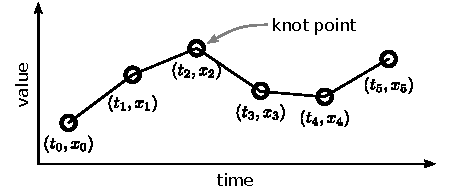
\includegraphics{fig/linearSpline.pdf}
  \caption{Linear Spline. We represent the dose-rate and leaf position trajectories as linear
           splines. A linear spline is fully defined by its value at the knot points. }
  \label{fig:linearSpline}
\end{figure}

\subsection{Trajectory Limits}

There are several constraints imposed on the dose-rate and leaf trajectories
by the physical limitations of the VMAT machine. Specifically, there is a maximum dose-rate,
constant limits on the leaf positions, and an upper limit on the leaf speed.
These limits are detailed below, where $\dot{z}(t) = \tfrac{d}{dt}z(t)$ gives the leaf velocity.
\begin{align}
  \text{dose-rate: }& \quad 0 \leq r(t) \leq r_\text{max}
      \label{eqn:FirstTrajectoryConstraint}\\
  \text{leaf position: }& \quad x_\text{min} \leq z_L(t) \leq z_U(t) \leq x_\text{max} \\
  \text{lower leaf velocity: }& \quad v_\text{min} \leq \dot{z}_L(t) \leq v_\text{max} \\
  \text{upper leaf velocity: }& \quad v_\text{min} \leq \dot{z}_U(t) \leq v_\text{max}
      \label{eqn:LastTrajectoryConstraint}
\end{align}

\subsection{Avoiding Local Minima}

One of the key issues with fluence mapping is that the
optimization tends to get stuck in local minima,
since there are a large number of leaf trajectories that deliver the same fluence to the target.
\addref{local minima in fluence mapping}

It is possible to help the optimization avoid local minima by smoothing the optimization problem.
This smoothing is useful because it means that the gradient estimates in the optimization change less
between each iteration in the optimization.

There is an obvious trade-off here: smoothing makes the optimization easier by fundamentally changing the problem statement,
thus we get an easy optimization that is inaccurate.
The solution here is to iteratively reduce the smoothing terms,
initially solving the optimization with heavy smoothing to avoid local minima,
and then using that solution to initialize another optimization with less smoothing.
See \S Section \ref{sec:modelingFluenceBlocking} for details.

This technique of iteratively reducing a smoothing term is widely used in trajectory optimization,
such is in \cite{Srinivasan2006}.


\subsection{Computing Delivered Fluence}

The fluence delivered at each position on the target is computed by integrating the
dose-rate function over the periods of time when the leaves are not blocking the target:

\begin{equation}
  f_D(x) = \int_{\mathcal{T}(x)} \! r(t) \,dt
  \quad \quad
  \mathcal{T}(x) = \forall t
  \quad
  \text{S.T.}
  \quad
  z_L(t) \leq x \leq z_U(t)
  \label{eqn:fluenceMapIntegral}
\end{equation}

There are two issues with computing this integral directory.
The first is that it requires either computing the inverse of the leaf trajectories,
which ultimately reduces to a non-linear root finding sub-problem.
When placed inside of an optimization, this will dramatically slow convergence.
The second issue is that the set $\mathcal{T}(x)$ does not smoothly vary with respect to the leaf trajectories.
It is possible to construct a set of leaf trajectories for which a small change in leaf position
switches $\mathcal{T}(x)$ from one to two simply connected sets.
Inside of an optimization, this would cause a change in the sparsity pattern of the gradient
(\textit{e.g.} $\tfrac{\partial f_D}{\partial z_L})$)
between successive iterations,
which leads to poor convergence and possibly a numerical instability.

Our solution is to rewrite the integral using a blocking function $k(t)$,
which has a value of one when the leaves are passing radiation and
zero when the leaves are blocking radiation, as described in \S\ref{sec:modelingFluenceBlocking}
This allows us to rewrite (\ref{eqn:fluenceMapIntegral}) using the constant bounds $[0, \mathcal{T}]$:

\begin{equation}
  f_D(x) = \int_0^T \! k(t, x) \cdot r(t) \, dt
  \label{eqn:fluenceDoseSimpleBounds}
\end{equation}

Now we have a standard scalar integral, where the integrand is smooth and the
bounds are constant, we can use any quadrature method to evaluate (\ref{eqn:fluenceDoseSimpleBounds}).
In this case we use the midpoint (rectangle) quadrature rule.

\subsection{Modeling Fluence Blocking}
\label{sec:modelingFluenceBlocking}

A simple way to define the fluence blocking function $k(t)$
would be to set it to one if $z_L(t) \leq x \leq z_U(t)$
is true, and zero otherwise.
This implementation would have a discontinuous gradient, which would cause problems in the optimization.
Instead, we use exponential smoothing to approximate the step function $s(x,\alpha)$,
where $\alpha$ is a small smoothing parameter.
A smaller smoothing parameter will provide a more accurate model,
while a larger smoothing parameter will lead to faster optimization.

\begin{equation}
  k(t, x) = \sqrt{s\big(x - z_L(t), \, \alpha\big) \; \cdot \; s\big(z_U(t) - z, \, \alpha\big)}
\end{equation}

\begin{equation}
  s(t, \alpha) = \frac{1}{1 + e^{-t/\alpha}}
\end{equation}

In practice it is useful to define the smoothing parameter $\alpha$ in terms of a smoothing distance ($\gamma$)
and the fraction change ($\Delta s$) in smoothing over this distance.

There is a physical interpretation of the smoothing distance $\gamma$ for the leaf-blocking model:
it is the distance, centered on the edge of the leaf, where the edge is blurred by the smoothing.

\begin{equation}
  \alpha = \frac{2}{\Delta s} \ln \left( \frac{1}{2} (1 - \gamma) \right)
\end{equation}


\subsection{Objective Function}

The objective function for the inner optimization (computing leaf trajectories)
is the integral of the error-squared between the target fluence $f_T(x)$ and the delivered fluence $f_D(x)$.
\begin{equation}
  J = \int_{x_\text{min}}^{x_\text{max}} \! \big( f_T(x) - f_D(x) \big)^2 \,dx
  \label{eqn:continuousFittingObjective}
\end{equation}

In practice we can only compute the fluence profile at a finite number of points.
We will break the domain $[x_\text{min}, x_\text{max}]$ into $N_\text{fit}$ equal-width segments,
and evaluate the fluence target and delivered fluence at the midpoint $x_k$ of each segment.
This is equivalent to approximating (\ref{eqn:continuousFittingObjective}) using rectangle (mid-point)
quadrature with $N_\text{fit}$ segments.

\begin{equation}
  J \approx \frac{x_\text{max} - x_\text{min}}{N_\text{fit}}\sum_{k = 1}^{N_\text{fit}} \! \big( f_T(x_k) - f_D(x_k) \big)^2
  \label{eqn:discreteFittingObjective}
\end{equation}

\subsection{Transcription to a Nonlinear Program}

The inner optimization loop computes the leaf trajectories $z_L(t)$ and $z_U(t)$
that minimize the objective function (\ref{eqn:FluenceFittingObjective})
and satisfy the constraints (\ref{eqn:FirstTrajectoryConstraint}--\ref{eqn:LastTrajectoryConstraint}).

The limits on leaf position can be implemented as a combination of
constant bounds and linear inequality constraints:

\begin{equation}
  x_\text{min} \leq x_{L, k}
  \quad \quad
  x_{U, k} \leq x_\text{max}
  \quad \quad
  x_{L, k} \leq x_{U, k}
  \quad \quad
  \forall k
\end{equation}

Since we represent these trajectories as piecewise linear,
it is natural to represent them by their values at the knot points $t_i$.
The position trajectory is piecewise linear,
and we can compute the velocity trajectory by taking the derivative of the spline.
The velocity between each pair of knot points will be constant and given by:

\begin{equation}
  \dot{z}_{L, k} = \frac{z_{L, k+1} - z_{L, k}}{h_k}
  \quad \quad
  \dot{z}_{U, k} = \frac{z_{U, k+1} - z_{U, k}}{h_k}
\end{equation}

The limits on velocity can thus be written as linear inequality constraints:

\begin{equation}
  v_\text{min} \leq \dot{z}_{L, k} \leq v_\text{max}
  \quad \quad
  v_\text{min} \leq \dot{z}_{U, k} \leq v_\text{max}
  \quad \quad \forall k
\end{equation}

\todo{Add a summary sentence about how to pack everything up into a NLP solver}


%~~~~~~~~~~~~~~~~~~~~~~~~~~~~~~~~~~~~~~~~~~~~~~~~~~~~~~~~~~~~~~~~~~~~~~~~~~~~~~~~~~~~~~~~~~~~~~~~~%


\section{Method - Outer Optimization - Dose Rate Trajectories}

\todo{Write this section.}

Proposed Method (yet to be tested):  Start by running CMAES witha wide search and heavy smoothing
parameters. Optimize over the smoothed objective at the low level, but then spend the extra CPU
time to benchmark the actual value of each solution. Once this optimization converges, then
run a second round of CMAES using iterative smoothing refinement.

\subsection{Objective Function:}

Best leaf trajectories!

\todo{Finish writing}

\subsection{Optimization:}

CMAES
\todo{Finish writing}
